\subsection{Vereinzelung} \label{sec:Inbetriebnahme_Vereinzelung}
Für die Parametrisierung der Bewegungsabläufe, sowie die Reglerauslegung wurde die Software ION Studio (siehe Abb. \ref{fig:ION_Studio}) verwendet. ION Studio kann auf einem Windows Rechner installiert werden und über USB mit dem ION Motion Roboclaw Motorencontroller verbunden werden. Sobald die Verbindung aufgebaut wurde, kann der Motorencontroller mit dem vollen Befehlsumfang angesteuerte werden. Dabei können Motorenparameter wie Strom, Drehzahl und Position grafisch analysiert werden. Bewegungsabläufe können so schnell und einfach analysiert, getestet und anschliessend in die Software des FRDM-Boards adaptiert werden.

\begin{figure}[H]
	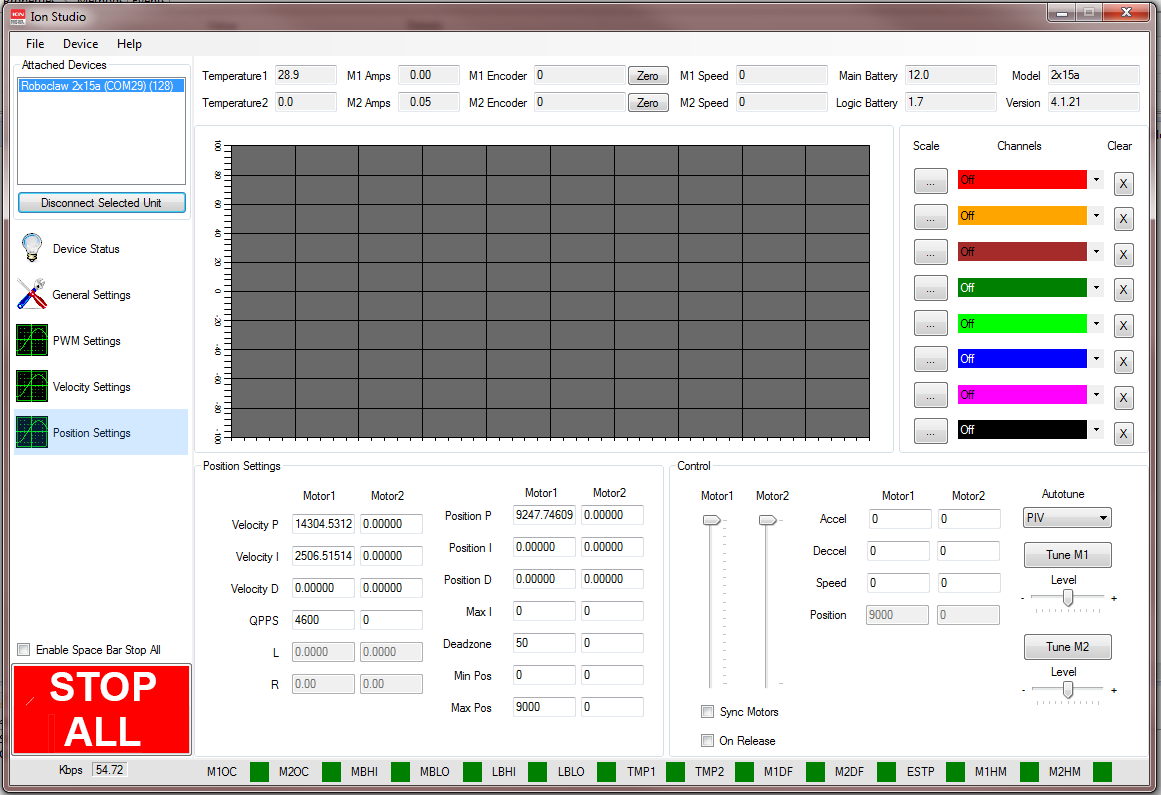
\includegraphics[draft=false,width=0.7\textwidth]{Illustrationen/7-Inbetriebnahme_und_Kalibration/ION_Studio.png}
	\caption{Benutzeroberfläche ION Studio}
	\label{fig:ION_Studio}
\end{figure}

Bei der Inbetriebnahme der Vereinzelung führte das grosse Getriebespiel des Pololu Motors zu einem beträchtlichen Problem. Da die Getriebeausgangswelle direkt die Lochmaske der Vereinzlung antreibt, überträgt sich dieses Spiel 1:1 auf den Mechanismus. Das Getriebespiel führte dazu, dass die Lochmaske nicht genau positioniert werden konnte. Dieses Problem konnte komplett gelöst werden, indem die Lochmaske während der Rotationsbewegung abgebremst wurde. Dadurch wurde ein Lastwechsel des Motors vermieden und das Spiel kam nicht zum tragen. Die Lochmaske konnte durch die Verwendung der Abstreifbürsten gebremst werden. Dabei wurden diese in der Länge gekürzt um eine optimale Bremsung zu erreichen ohne den Motor zu stark zu belasten. In Abb. \ref{fig:spiel_lochmaske} ist das Resultat dieser Massnahme sichtbar.

\begin{figure}[H]
	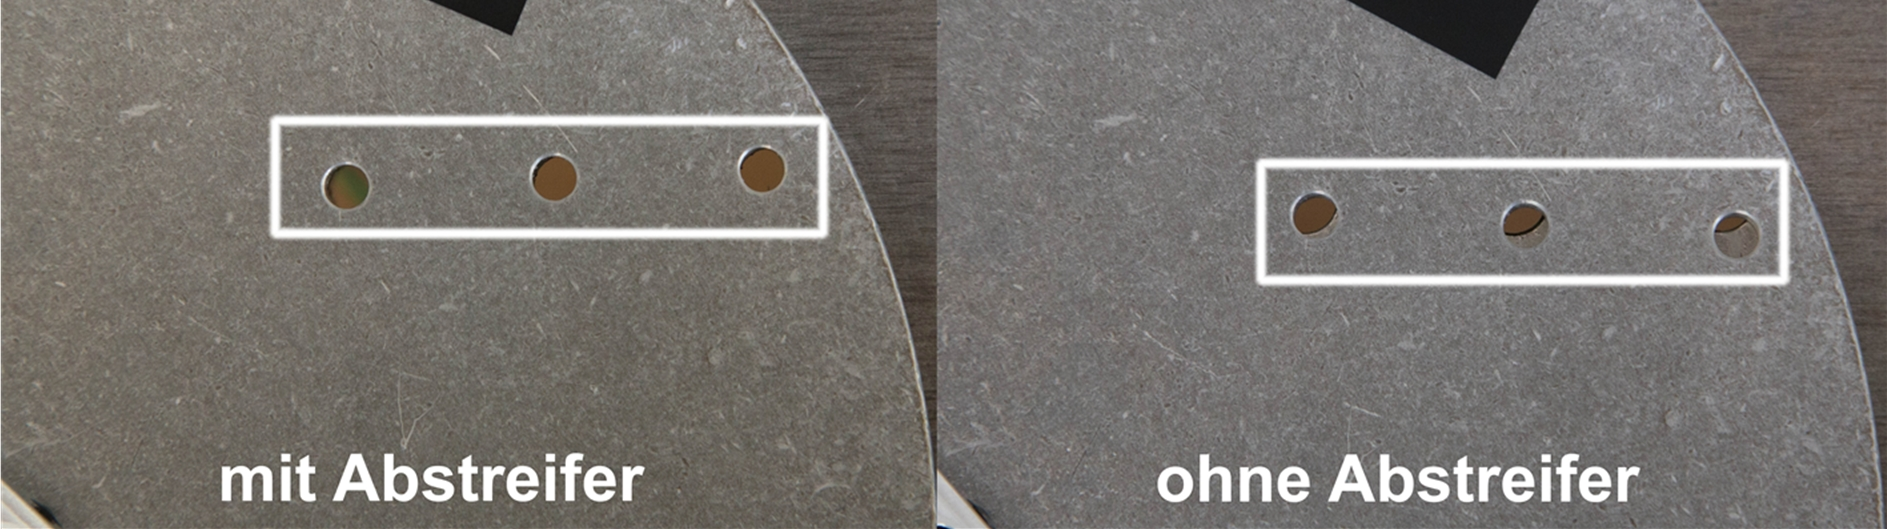
\includegraphics[draft=false,width=1\textwidth]{Illustrationen/7-Inbetriebnahme_und_Kalibration/spiel_lochmaske_1.jpg}
	\caption{Spiel der Lochmaske mit und ohne Abstreifer}
	\label{fig:spiel_lochmaske}
\end{figure}

Eine weitere Massnahme zur Verbesserung der Positionierungsgenauigkeit der Vereinzelung war die Verwendung des 1:378 Getriebemotors, welcher für die Verstellmechanik evaluiert wurde. Dieser kann aufgrund des grösseren Getriebes präziser positioniert werden. Der Parameter für die Encodercounts des Offsets (-1700) wurde experimentell ermittelt. Die Schrittweite zwischen den Lochmasken wurde errechnet. Die Anzahl Encoder Counts für eine ganze Umdrehung der Getriebeausgangswelle beträgt 18,140. Dabei sind auf der Lochmaske 6 Lochbilder in gleichmässigen Abstand ausgeführt. Demensprechend beträgt die Anzahl Encoder Counts pro Schrittweite ca. 3025. Die PID Parameter der Positionierungsregelung wurden durch die Autotune Funktion des Motorencontrollers bestimmt.
\newline

Mit den umgesetzten Massnahmen wurde die Vereinzelung getestet. Die Vereinzelung von NemaCaps erfolgt zuverlässig. Nur in der Minderheit der Fälle (<15\%) bleibt das NemaCap an der Lochmaske hängen. Weiter muss beachtet werden, dass die Mindestfüllhöhe der Trommel nicht unterschritten wird.
\newline

Um die Zuverlässigkeit weiter zu steigern, sind die genannten Abhilfemassnahmen in Betrieb zu nehmen (vgl. Kap. \ref{abhilfe}). Diese konnten mangels Zeit nicht implementiert werden.
\subsubsection{Entleeren}
\textit{(ygu)} Weiter wurde das Entleeren der Trommel getestet. Abbildung \ref{fig:entleeren} illustriert diesen Vorgang:

\begin{figure}[H]
	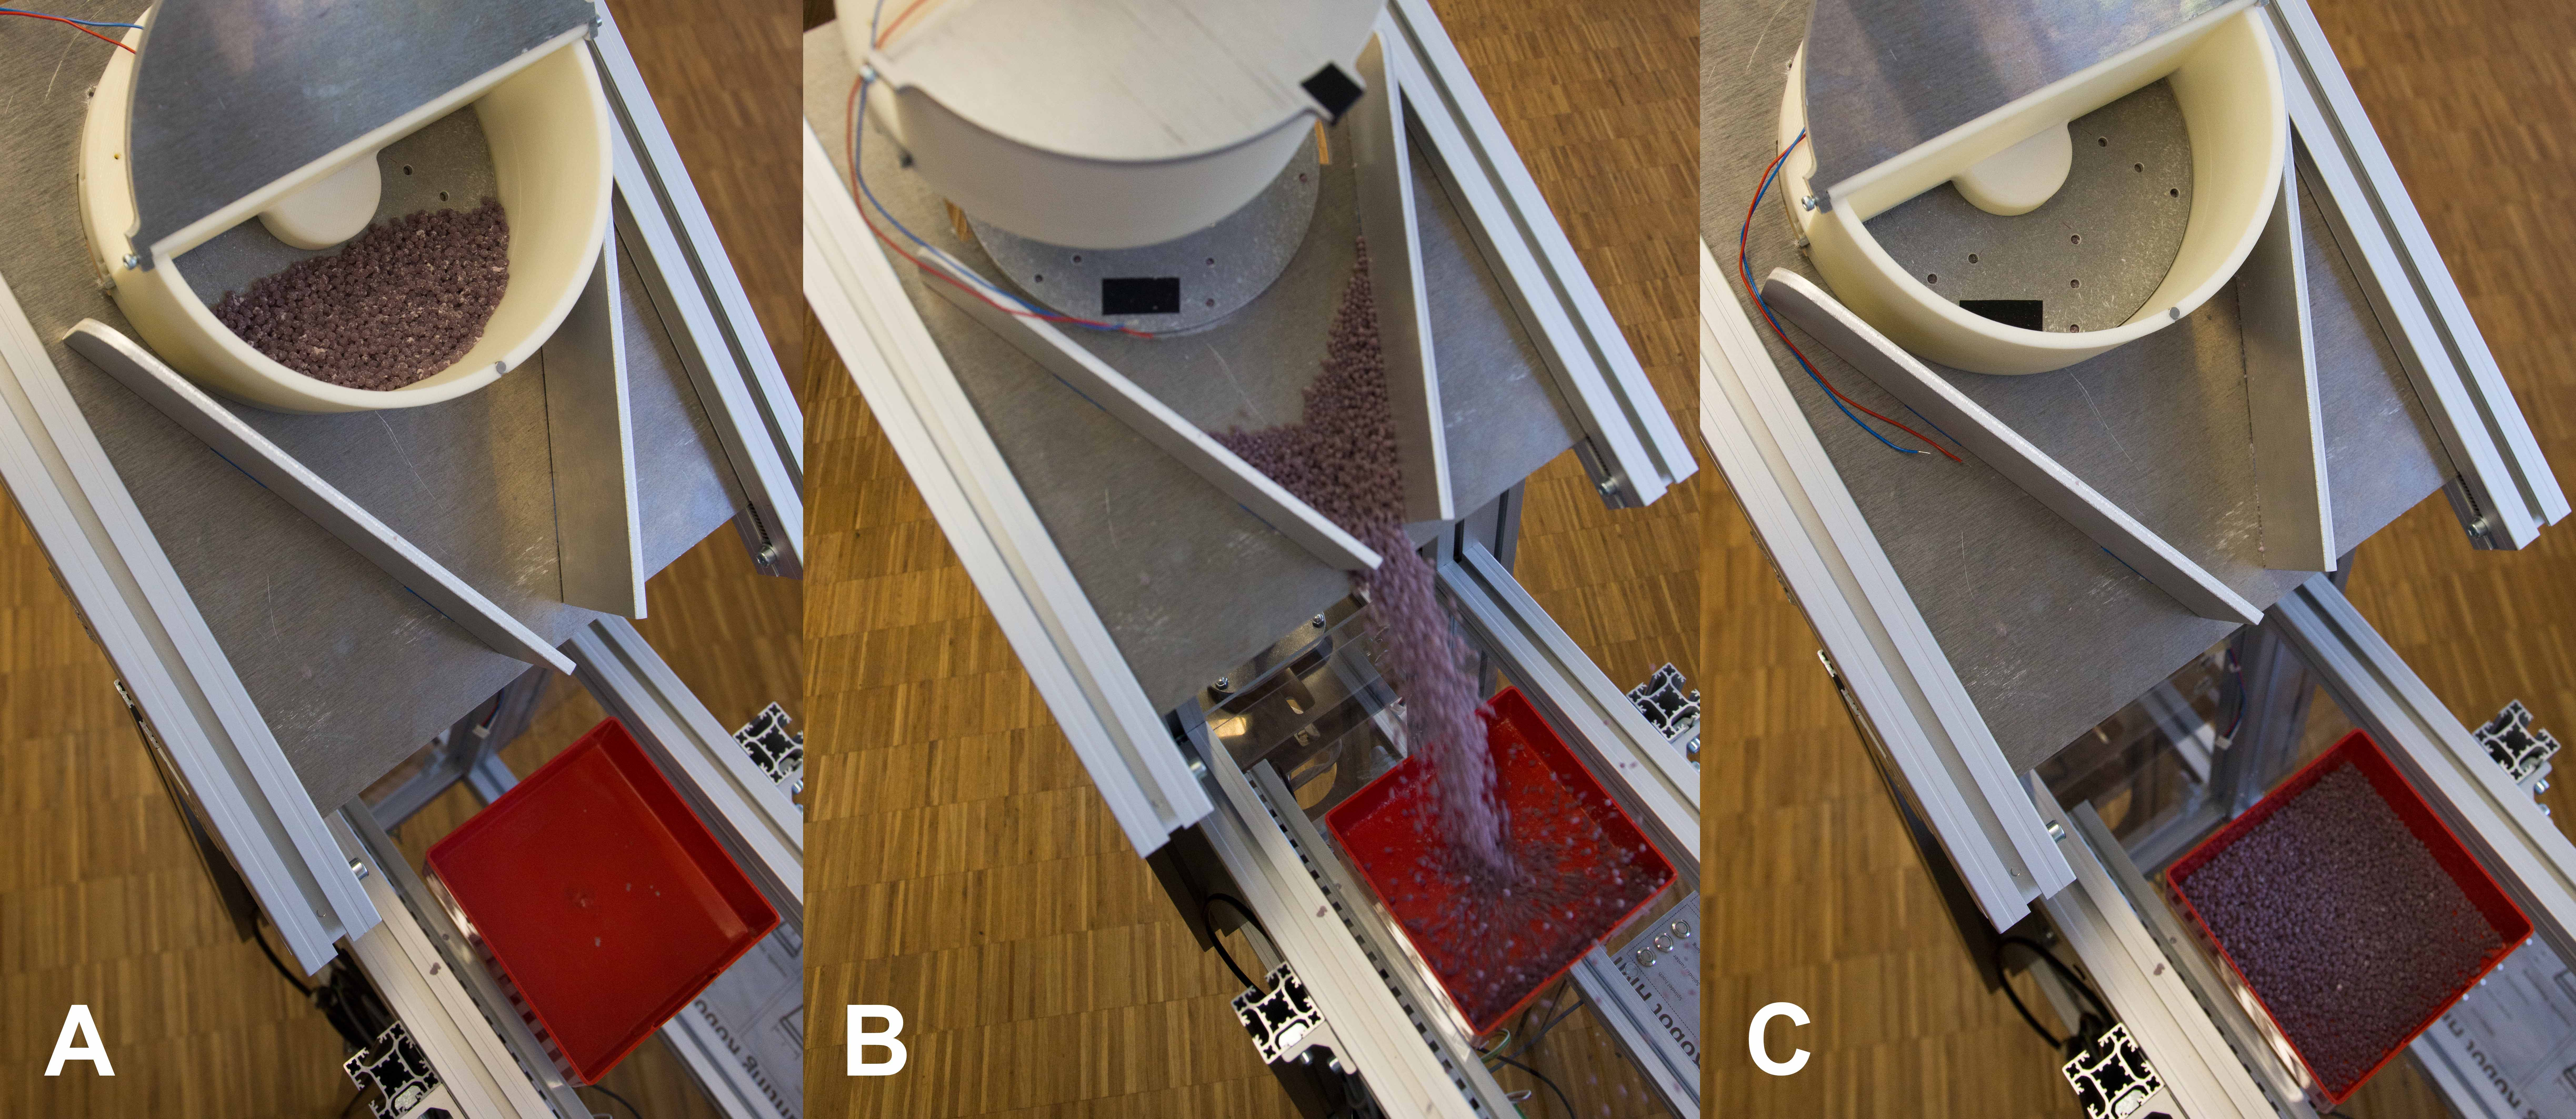
\includegraphics[draft=false,width=1\textwidth]{Illustrationen/7-Inbetriebnahme_und_Kalibration/entleeren.jpg}
	\caption{Entleerung der Trommel}
	\label{fig:entleeren}
\end{figure}

Mit einer Drehung der Trommel um 15° wird der Bajonettverschluss entriegelt und die Trommel kann entfernt werden (Phase B in Abb. \ref{fig:entleeren}). Sogleich rollen die NemaCaps zur Öffnung und fallen in den vorgesehenen Behälter. Die umgesetzte Entleerung funktioniert ohne Komplikationen und steigert die Benutzerfreundlichkeit massgebend.